
\section{Durchführung}
Zur Durchführung des Versuchs wird ein RC-Kreis wie in Abb. \ref{fig:aufbau} aufgebaut. Mithilfe
eines Oszilloskops kann der Auf- und Entladedevorgang des Kondensators beobachtet werden.
Hierfür wird mit dem Generator eine Rechteckspannung angelegt.
\begin{figure}
  \centering
  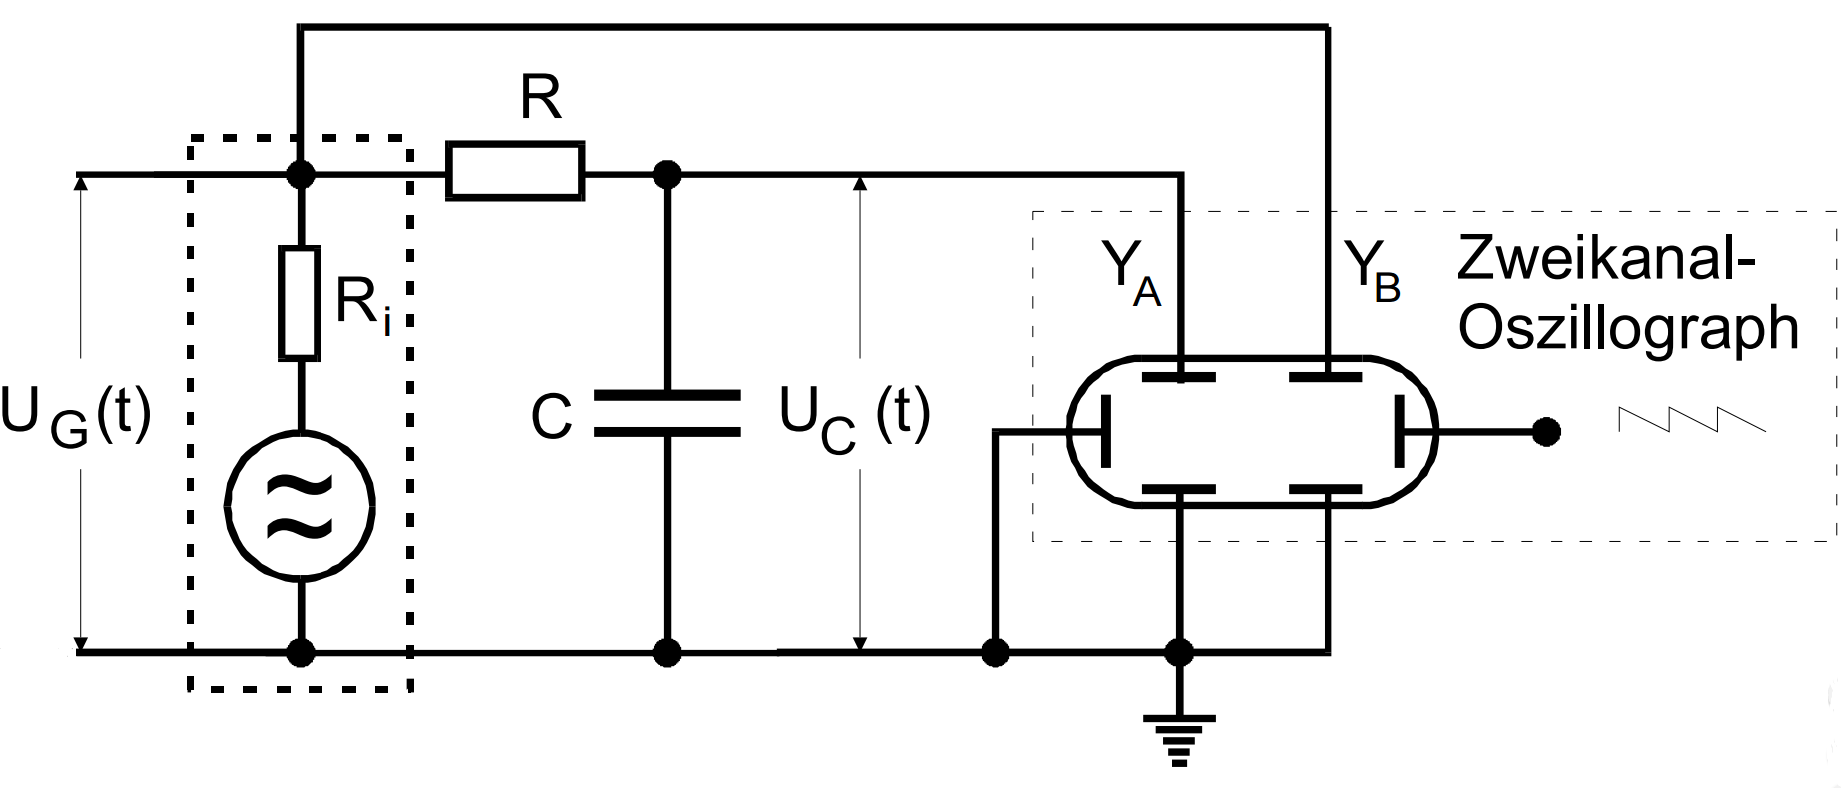
\includegraphics[width = \textwidth]{Aufbau_V353.png}
  \caption{Aufbau des RC-Kreis für die unterschiedlichen Messungen.}
  \label{fig:aufbau}
\end{figure}

Im Folgenden wird der Generator auf eine Sinusspannung umgestellt.
Über einen Frequenzbereich
von 10Hz bis 30Hz wird die Spannungsamplitude, abhänigig von der Zeit $t$
, am Kondensator bestimmt.

Des weiteren wird die Phasenverschiebung zwischen Generator- und Kondensatorspannung
in Abhänigkeit von der Frequenz ermittelt. Dafür werden beide Eingänge des Oszilloskops verwendet.
Hierbei ist zu beachten, dass beide Sinuskurven symmetrisch zur x-Achse liegen. Es gilt die
beiden Nulldurchgänge der Schwingungen und die Schwingungsdauer zu bestimmen. Daraus kann die
Phasenverschiebung $\phi$ mit
\begin{equation}
\varphi = \frac{a}{b} 2 \pi.
\label{eqn:phi}
\end{equation}
berechnet werden.

Um die Funktion des RC-Kreis als Integrator zu zeigen
werden eine Rechteck-,
Sinus- und Dreiecksspannung bei unterschiedlichen Frequenzen untersucht.
